\documentclass{article}
\usepackage{amsmath}
\usepackage{amssymb}
\usepackage{galois}
\usepackage{tikz}
\usepackage{stmaryrd}
\usepackage{tkz-euclide}
\usepackage{pgfplots}
\pgfplotsset{compat=newest} 
\newcommand{\envplus}{\textrm{Env}^+}
\newcommand{\envcirc}{\textrm{Env}^{\circ}}
\newcommand{\envsharp}{\textrm{Env}^{\#}}
\newcommand{\stateplus}{\textrm{State}^+}
\newcommand{\statecirc}{\textrm{State}^{\circ}}
\newcommand{\statesharp}{\textrm{State}^{\#}}
\newcommand{\cvplus}{\textrm{ContextVec}^+}
\newcommand{\cvcirc}{\textrm{ContextVec}^{\circ}}
\newcommand{\cvsharp}{\textrm{ContextVec}^{\#}}
\newcommand{\posetOf}[2]{\langle #1,\subseteq^{#2},\sqcup^{#2},\sqcap^{#2},\perp^{#2},\top^{#2}\rangle}
\begin{document}

Un \textit{environment} \(e^{\circ}\in\mathrm{Env}^{\circ}\triangleq \mathrm{Id}\rightarrow \mathrm{Value}\) è una funzione totale che mappa ogni variabile \(id \in\textrm{Id}\) ad un valore \(v\in\textrm{Value}\). Può essere visualizzato così:

\[
  \left[
  \begin{array}{ccl}
  id_1 &\longrightarrow &v_1 \\
  id_2 &\longrightarrow &v_2 \\
      &\cdots          &  \\
  id_n &\longrightarrow &v_n
  \end{array}
  \right]
\]


Un \textit{environment} \(e^{+}\in\mathrm{Env}^{+}\triangleq \mathrm{Id}\rightarrow \wp(\mathrm{Value})\) è una funzione totale che mappa ogni variabile \(id \in\textrm{Id}\) ad un insieme di valori  \(V\subseteq\textrm{Value}\). Può essere visualizzato così:

\[
  \left[
  \begin{array}{ccc}
  id_1 &\longrightarrow &\{v_1, \cdots, v_i\} \\
  id_2 &\longrightarrow &\{v_n, \cdots, v_m\} \\
      &\cdots          &  \\
  id_n &\longrightarrow &\{v_j, \cdots, v_k\}
  \end{array}
  \right]
\]

Possiamo ora creare i reticoli:
\begin{itemize}
\item 
\( L^{\circ}\triangleq
\langle 
	\wp(\textrm{Env}^{\circ}),
	\subseteq^{\circ},
	\sqcup^{\circ},
	\sqcap^{\circ},
	\perp^{\circ},
	\top^{\circ},
\rangle\)
dove 
\begin{itemize}
	\item \(\subseteq^{\circ}\) è il normale ordinamento di contenimento tra insiemi \(\subseteq\);
	\item \(\sqcup^{\circ}\) è l'operatore di unione  tra insiemi \(\cup\) e funge da \textit{lub};
	\item \(\sqcap^{\circ}\) è l'operatore di intersezione tra insiemi \(\cap\) e funge da \textit{glb};
	\item \(\perp^{\circ}\) è l'elemento \textit{bottom} del reticolo ed è l'insieme vuoto \(\varnothing\);
	\item \(\top^{\circ}\) è l'elemento \textit{top} del reticolo ed è tutto l'insieme \(\textrm{Env}^{\circ}\);	
\end{itemize}
\item \(L^{+}\triangleq
\langle
	\textrm{Env}^{+}, 
	\subseteq^{+},
	\sqcup^{+},
	\sqcap^{+},
	\perp^{+},
	\top^{+},
\rangle\) dove:
\begin{itemize}
	\item \(\subseteq^{+}\) è un \textit{ordinamento parziale} su \(\textrm{Env}^{+}\). Dati \(e^+_1, e^+_2 \in\textrm{Env}^+\) abbiamo: 
	\[ e^+_1\subseteq^{+} e^+_2 \textrm{ se e solo se } \forall id\in\textrm{Id}.\ e^+_1[id]\subseteq e^+_2[id]\]
	\item \(\sqcup^{+}\) è l'operatore di \textit{lub}. Dati \(e^+_1, e^+_2 \in\textrm{Env}^+\) abbiamo
	\[ e^+_1\sqcup^{+} e^+_2 = \lambda id.\  e^+_1[id]\cup e^+_2[id]\]
	\item \(\sqcap^{+}\) è l'operatore di \textit{glb}. Dati \(e^+_1, e^+_2 \in\textrm{Env}^+\) abbiamo
	\[ e^+_1\sqcup^{+} e^+_2 = \lambda id.\  e^+_1[id]\cap e^+_2[id]\]
	\item \(\perp^{+}\) è l'elemento \textit{bottom} del reticolo ed è quell'elemento \(e^+\in\textrm{Env}^+\) tale che \(\forall id\in\textrm{Id}.\  e^+[id] = \varnothing\);
	\item \(\top^{+}\) è l'elemento \textit{top} del reticolo ed è quell'elemento \(e^+\in\textrm{Env}^+\) tale che \(\forall id\in\textrm{Id}.\  e^+[id] = \textrm{Value}\);
\end{itemize}
\end{itemize}

E' possibile costruire una \textit{connessione di Galois}:  \[
	\langle 
	\wp(\envcirc), 
	\subseteq^{\circ}
	\rangle 
\galois
{\alpha^{\circ\rightarrow +}}
{\gamma^{+ \rightarrow\circ}} 
	\langle 
	\envplus, 
	\subseteq^+
	\rangle
\]
dove: 
\begin{itemize}
\item \(\alpha^{\circ\rightarrow +} : \wp(\envcirc)\rightarrow\envplus\) è la \textit{funzione di astrazione}. Dato \(env^{\circ} \in \wp(\envcirc)\) abbiamo che:
\[\alpha^{\circ\rightarrow +}(env^{\circ}) = \lambda id.\ \{v \in\textrm{Value}\ \vert\ \exists e^{\circ}\in env^{\circ}.\ e^{\circ}[id] = v\}\]
\item \(\gamma^{+ \rightarrow\circ} : \envplus\rightarrow\wp(\envcirc)\) è la \textit{funzione di concretizzazione}. Dato \(e^+ \in \envplus\) abbiamo che:
\[\gamma^{+ \rightarrow\circ}(e^+) = \{e^{\circ} \in\envcirc\ \vert\ \forall id\in\textrm{Id}, e^{\circ}[id]\in e^+[id]\}\]
\end{itemize}

Supponiamo ora di avere un reticolo  \(V^{\#}\triangleq\posetOf{\textrm{Value}^{\#}}{\ast}\) che astrae il reticolo  \(V\triangleq\langle\wp(\textrm{Value}),\subseteq,\cup,\cap,\varnothing,\textrm{Value}\rangle\) ovvero è possibile definire una connessione di Galois:
\[
	\langle\wp(\textrm{Value}), \subseteq\rangle
	\galois{\alpha^{\#}}{\gamma^{\#}}
	\langle\textrm{Value}^{\#}, \subseteq^{\ast}\rangle
\]

Un \textit{environment} \(e^{\#}\in\envsharp\triangleq \mathrm{Id}\rightarrow \textrm{Value}^{\#}\) è una funzione totale che mappa ogni variabile \(id \in\textrm{Id}\) ad un valore \(v^{\#}\in\textrm{Value}^{\#}\). Può essere visualizzato così:
\[
  \left[
  \begin{array}{ccl}
  id_1 &\longrightarrow &v^{\#}_1 \\
  id_2 &\longrightarrow &v^{\#}_2 \\
      &\cdots          &  \\
  id_n &\longrightarrow &v^{\#}_n
  \end{array}
  \right]
\]

Emerge il reticolo
\(L^{\ast}\triangleq \posetOf{\textrm{Env}^{\#}}{\#}\) dove:
\begin{itemize}
	\item \(\subseteq^{\#}\) è un \textit{ordinamento parziale} su \(\textrm{Env}^{\#}\). Dati \(e^{\#}_1, e^{\#}_2 \in\textrm{Env}^{\#}\) abbiamo: 
	\[ e^{\#}_1\subseteq^{+} e^{\#}_2 \textrm{ se e solo se } \forall id\in\textrm{Id}:e^{\#}_1[id]\subseteq^{\ast} e^{\#}_2[id]\]
	\item \(\sqcup^{\#}\) è l'operatore di \textit{lub}. Dati \(e^{\#}_1, e^{\#}_2 \in\textrm{Env}^{\#}\) abbiamo
	\[ e^{\#}_1\sqcup^{\#} e^{\#}_2 = \lambda id.\  e^{\#}_1[id]\cup^{\ast} e^{\#}_2[id]\]
	\item \(\sqcap^{\#}\) è l'operatore di \textit{glb}. Dati \(e^{\#}_1, e^{\#}_2 \in\textrm{Env}^{\#}\) abbiamo
	\[ e^{\#}_1\sqcup^{\#} e^{\#}_2 = \lambda id.\  e^{\#}_1[id]\cap^{\ast} e^{\#}_2[id]\]
	\item \(\perp^{\#}\) è l'elemento \textit{bottom} del reticolo ed è quell'elemento \(e^{\ast}\in\textrm{Env}^{\#}\) tale che \(\forall id\in\textrm{Id}.\  e^{\#}[id] = \perp^{\ast}\);
	\item \(\top^{\#}\) è l'elemento \textit{top} del reticolo ed è quell'elemento \(e^{\ast}\in\textrm{Env}^{\#}\) tale che \(\forall id\in\textrm{Id}.\  e^{\#}[id] = \top^{\ast}\);
\end{itemize}

E' possibile ora costruire una connessione di Galois:
\[
\langle
	\envplus,
	\subseteq^+
\rangle
\galois
	{\alpha^{+\rightarrow\#}}
	{\gamma^{\#\rightarrow +}}
\langle
	\envsharp,
	\subseteq^{\#}
\rangle
\]
dove: 
\begin{itemize}
\item \(\alpha^{+\rightarrow\#} : \envplus\rightarrow\envsharp\) è la \textit{funzione di astrazione}. Dato \(e^+ \in \envplus\) abbiamo che:
\[\alpha^{+\rightarrow\#}(e^+) = \lambda id.\ \{v^{\#} \in\textrm{Value}^{\#}\ \vert\ \bigsqcup^{\#}\{\alpha^{\#}(v)\ \vert\ v\in e^+[id]\}\}\]
\item \(\gamma^{\#\rightarrow +} : \envsharp\rightarrow\envplus\) è la \textit{funzione di concretizzazione}. Dato \(e^{\#} \in \envsharp\) abbiamo che:
\[\gamma^{\#\rightarrow +}(e^{\#}) = \lambda id.\ \gamma^{\#}(e^{\#}[id])\]
\end{itemize}

Supponiamo che \(\textrm{Value} = \mathbb{Z}^+\) e che \(\textrm{Id}=\{x, y\}\). Un \(e^{\circ}\in\envcirc\) è una funzione che mappa \(x\textrm{ e } y\) ad un valore intero positivo. \(e^{\circ}\) può anche essere visto come una coppia di valori \((x, y)\) dove \(x, y\in\mathbb{Z}^+\) e perciò \(e^{\circ}\) è un punto nel piano cartesiano in due dimensioni.
Quindi \(envs^{\circ}\in\wp(\envcirc)\) è un insieme di punti nel piano cartesiano. Per fare un esempio: 

\begin{align*}
envs^{\circ} = \{&(1,1),(1,2),(1,3),(2,5),	\\		   &(2,3),(2,2),(4,1),(4,2)\}
\end{align*}
\begin{center}
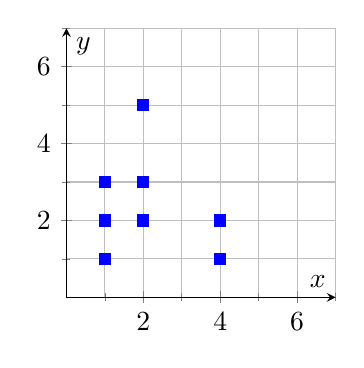
\begin{tikzpicture}
\begin{axis}[
axis lines=middle,
axis equal,
xlabel = \(x\),
ylabel = \(y\),
xmin=0, xmax=7,
ymin=0, ymax=7,
width=5cm,height=5cm,
grid=both,
minor tick num=1]
\addplot[color=blue,mark=square*,only marks]
    coordinates {(1,1)(1,2)(1,3)(2,5)
    (2, 3)(2,2)(4,1)(4,2)};
\end{axis}
\end{tikzpicture}
\end{center}

Se applichiamo la funzione di astrazione \(\alpha^{\circ\rightarrow +}\) a \(envs^{\circ}\) si ottiene:
\[
  \alpha^{\circ\rightarrow +}(envs^{\circ}) =
  e^+ = 
  \left[
  \begin{array}{ccc}
  x &\longrightarrow &\{1, 2, 4\} \\
  y &\longrightarrow &\{1, 2, 3, 5\}
  \end{array}
  \right]
\]
\begin{center}
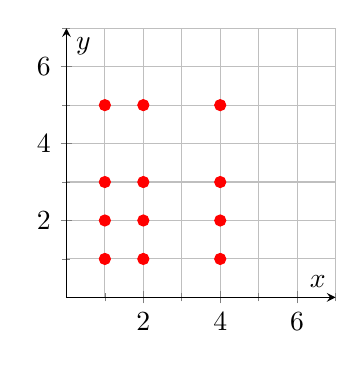
\begin{tikzpicture}
\begin{axis}[
axis lines=middle,
axis equal,
xlabel = \(x\),
ylabel = \(y\),
xmin=0, xmax=7,
ymin=0, ymax=7,
width=5cm,height=5cm,
grid=both,
minor tick num=1]
\addplot[color=red,mark=*,only marks]
    coordinates {
    (1,1)(1,2)(1,3)(1,5)
    (2,1)(2,5)(2,3)(2,2)
    (4,1)(4,2)(4,3)(4,5)};
\end{axis}
\end{tikzpicture}
\end{center}

Come si può vedere c'è una perdita di informazione. In particolare si perde il concetto di relazione tra i valori delle variabili. Cioè il valore di una variabile è indipendente dal valore delle altre variabili.

Se come dominio astratto \(\textrm{Value}^{\#}\) prendiamo il dominio degli intervalli e definiamo una funzione di astrazione e una di concretizzazione tale da creare una connessione di Galois:
 \[\langle\envplus, \subseteq^+\rangle
\galois
	{\alpha^{+\rightarrow \textrm{Int}}}
	{\gamma^{\textrm{Int}\rightarrow +}}
	\langle\textrm{Int}, \subseteq^{\textrm{Int}}\rangle\]

possiamo trasformare un \(e^+\in\envplus\) in un \(e^{\textrm{Int}}\in\textrm{Env}^{\textrm{Int}}\):

\[
  \alpha^{+\rightarrow \textrm{Int}}(e^+) =
  e^{\textrm{Int}} = 
  \left[
  \begin{array}{ccc}
  x &\longrightarrow &[1,4] \\
  y &\longrightarrow &[1,5]
  \end{array}
  \right]
\]

\begin{center}
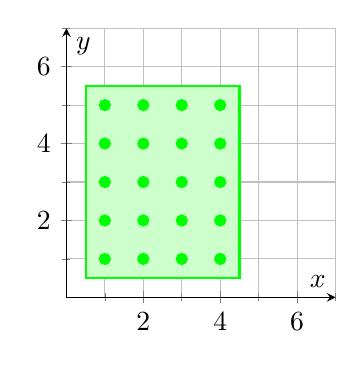
\begin{tikzpicture}
\begin{axis}[
axis lines=middle,
axis equal,
xlabel = \(x\),
ylabel = \(y\),
xmin=0, xmax=7,
ymin=0, ymax=7,
width=5cm,height=5cm,
grid=both,
minor tick num=1]
\draw[draw=green,fill=green!20, thick] (0.5,0.5) rectangle (4.5,5.5);
\addplot[color=green,mark=*,only marks]
    coordinates {
    (1,1)(1,2)(1,3)(1,4)(1,5)
    (2,1)(2,2)(2,3)(2,4)(2,5)
    (3,1)(3,2)(3,3)(3,4)(3,5)
    (4,1)(4,2)(4,3)(4,4)(4,5)};
\end{axis}
\end{tikzpicture}
\end{center}

Un \textit{context vectors} \(Cv^{\circ}\in\textrm{ContextVec}^{\circ}\triangleq\textrm{ProgramPoint}\rightarrow\wp(\envcirc)\) è una funzione totale che mappa ogni program point \(pp\in\textrm{ProgramPoint}\) ad un insieme di environment \(env^{\circ}\subseteq\envcirc\). Può essere visualizzato così:

\[
  \left[
  \begin{array}{ccc}
  pp_1 &\longrightarrow &
  	\left\{
  	\left[
  	\begin{array}{ccc}
  	id_1 &\longrightarrow &v_i \\
  	     &\cdots \\
  	id_m &\longrightarrow &v_j
  	\end{array}
  	\right], 
  	\cdots ,
  	\left[
  	\begin{array}{ccc}
  	id_1 &\longrightarrow &v_k \\
  	     &\cdots \\
  	id_m &\longrightarrow &v_l
  	\end{array}
  	\right] 
  	\right\}
   \\
    \vdots & &\vdots 
   \\
  pp_n &\longrightarrow &
  	\left\{
  	\left[
  	\begin{array}{ccc}
  	id_1 &\longrightarrow &v_m \\
  	     &\cdots \\
  	id_m &\longrightarrow &v_n
  	\end{array}
  	\right], 
  	\cdots ,
  	\left[
  	\begin{array}{ccc}
  	id_1 &\longrightarrow &v_t \\
  	     &\cdots \\
  	id_m &\longrightarrow &v_s
  	\end{array}
  	\right] 
  	\right\}
  \end{array}
  \right]
\]

Un \textit{context vectors} \(Cv^{+}\in\textrm{ContextVec}^{+}\triangleq\textrm{ProgramPoint}\rightarrow\envplus\) è una funzione totale che mappa ogni program point \(pp\in\textrm{ProgramPoint}\) ad un environment \(e^+\in\envplus\).

Un \textit{context vectors} \(Cv^{\#}\in\textrm{ContextVec}^{\#}\triangleq\textrm{ProgramPoint}\rightarrow\envsharp\) è una funzione totale che mappa ogni program point \(pp\in\textrm{ProgramPoint}\) ad un environment \(e^{\#}\in\envsharp\).

E' possibile definire tre reticoli:
\begin{itemize}
\item 
\( \widehat{L^{\circ}}\triangleq
\langle 
	\cvcirc,
	\widehat{\subseteq^{\circ}},
	\widehat{\sqcup^{\circ}},
	\widehat{\sqcap^{\circ}},
	\widehat{\perp^{\circ}},
	\widehat{\top^{\circ}},
\rangle\), 
dove 
\begin{itemize}
	\item \(\widehat{\subseteq^{\circ}}\) è un \textit{ordinamento parziale} su \(\cvcirc\). Dati \(Cv_1^{\circ}, Cv_2^{\circ}\in\cvcirc\) abbiamo:
	\[Cv_1^{\circ}\ \widehat{\subseteq^{\circ}}\ Cv_2^{\circ}\textrm{ se e solo se }\forall pp\in\textrm{ProgramPoint}.\ Cv_1^{\circ}[pp] \subseteq Cv_2^{\circ}[pp]\]
	\item \(\widehat{\sqcup^{\circ}}\) è l'operatore di \textit{lub}. Dati \(Cv_1^{\circ}, Cv_2^{\circ}\in\cvcirc\) abbiamo: 
	\[Cv_1^{\circ}\ \widehat{\sqcup^{\circ}}\ Cv_2^{\circ} = \lambda pp.\ Cv_1^{\circ}[pp] \cup Cv_2^{\circ}[pp]\]
	\item \(\widehat{\sqcap^{\circ}}\) è l'operatore di \textit{glb}. Dati \(Cv_1^{\circ}, Cv_2^{\circ}\in\cvcirc\) abbiamo: 
	\[Cv_1^{\circ}\ \widehat{\sqcap^{\circ}}\ Cv_2^{\circ} = \lambda pp.\ Cv_1^{\circ}[pp] \cap Cv_2^{\circ}[pp]\]
	\item \(\widehat{\perp^{\circ}}\ \) è l'elemento \textit{bottom} del reticolo ed è quell'elemento \(Cv^{\circ}\in\cvcirc\) tale che \(\forall pp \in\textrm{ProgramPoint}.\ Cv^{\circ}[pp] = \varnothing\);
	\item \(\widehat{\top^{\circ}}\ \) è l'elemento \textit{top} del reticolo ed è quell'elemento \(Cv^{\circ}\in\cvcirc\) tale che \(\forall pp \in\textrm{ProgramPoint}.\ Cv^{\circ}[pp] = \envcirc\);
\end{itemize}
\item 
\( \widehat{L^{+}}\triangleq
\langle 
	\cvplus,
	\widehat{\subseteq^{+}},
	\widehat{\sqcup^{+}},
	\widehat{\sqcap^{+}},
	\widehat{\perp^{+}},
	\widehat{\top^{+}},
\rangle\), 
dove 
\begin{itemize}
	\item \(\widehat{\subseteq^{+}}\) è un \textit{ordinamento parziale} su \(\cvplus\). Dati \(Cv_1^{+}, Cv_2^{+}\in\cvplus\) abbiamo:
	\[Cv_1^{+}\ \widehat{\subseteq^{+}}\ Cv_2^{+}\textrm{ se e solo se }\forall pp\in\textrm{ProgramPoint}.\ Cv_1^{+}[pp] \subseteq^+ Cv_2^{+}[pp]\]
	\item \(\widehat{\sqcup^{+}}\) è l'operatore di \textit{lub}. Dati \(Cv_1^{+}, Cv_2^{+}\in\cvplus\) abbiamo: 
	\[Cv_1^{+}\ \widehat{\sqcup^{+}}\ Cv_2^{+} = \lambda pp.\ Cv_1^{+}[pp] \sqcup^+ Cv_2^{+}[pp]\]
	\item \(\widehat{\sqcap^{+}}\) è l'operatore di \textit{glb}. Dati \(Cv_1^{+}, Cv_2^{+}\in\cvplus\) abbiamo: 
	\[Cv_1^{+}\ \widehat{\sqcap^{+}}\ Cv_2^{+} = \lambda pp.\ Cv_1^{+}[pp] \sqcap^+ Cv_2^{+}[pp]\]
	\item \(\widehat{\perp^{+}}\) è l'elemento \textit{bottom} del reticolo ed è quell'elemento \(Cv^{+}\in\cvplus\) tale che \(\forall pp \in\textrm{ProgramPoint}.\ Cv^{+}[pp] = \perp^+\);
	\item \(\widehat{\top^{+}}\ \) è l'elemento \textit{top} del reticolo ed è quell'elemento \(Cv^{+}\in\cvplus\) tale che \(\forall pp \in\textrm{ProgramPoint}.\ Cv^{+}[pp] = \top^+\);
\end{itemize}
\item 
\( \widehat{L^{\#}}\triangleq
\langle 
	\cvsharp,
	\widehat{\subseteq^{\#}},
	\widehat{\sqcup^{\#}},
	\widehat{\sqcap^{\#}},
	\widehat{\perp^{\#}},
	\widehat{\top^{\#}},
\rangle\), 
dove 
\begin{itemize}
	\item \(\widehat{\subseteq^{\#}}\) è un \textit{ordinamento parziale} su \(\cvsharp\). Dati \(Cv_1^{\#}, Cv_2^{\#}\in\cvsharp\) abbiamo:
	\[Cv_1^{\#}\ \widehat{\subseteq^{\#}}\ Cv_2^{\#}\textrm{ se e solo se }\forall pp\in\textrm{ProgramPoint}.\ Cv_1^{\#}[pp] \subseteq^+ Cv_2^{\#}[pp]\]
	\item \(\widehat{\sqcup^{\#}}\) è l'operatore di \textit{lub}. Dati \(Cv_1^{\#}, Cv_2^{\#}\in\cvsharp\) abbiamo: 
	\[Cv_1^{\#}\ \widehat{\sqcup^{\#}}\ Cv_2^{\#} = \lambda pp.\ Cv_1^{\#}[pp] \sqcup^{\#} Cv_2^{\#}[pp]\]
	\item \(\widehat{\sqcap^{\#}}\) è l'operatore di \textit{glb}. Dati \(Cv_1^{\#}, Cv_2^{\#}\in\cvsharp\) abbiamo: 
	\[Cv_1^{\#}\ \widehat{\sqcap^{\#}}\ Cv_2^{\#} = \lambda pp.\ Cv_1^{\#}[pp] \sqcap^{\#} Cv_2^{\#}[pp]\]
	\item \(\widehat{\perp^{\#}}\) è l'elemento \textit{bottom} del reticolo ed è quell'elemento \(Cv^{\#}\in\cvsharp\) tale che \(\forall pp \in\textrm{ProgramPoint}.\ Cv^{\#}[pp] = \perp^{\#}\);
	\item \(\widehat{\top^{\#}}\ \) è l'elemento \textit{top} del reticolo ed è quell'elemento \(Cv^{\#}\in\cvsharp\) tale che \(\forall pp \in\textrm{ProgramPoint}.\ Cv^{\#}[pp] = \top^{\#}\);
\end{itemize}
\end{itemize}

Possiamo notare come il dominio \(\envcirc\) sia fatto di elementi che indicano un \textit{environment} unico, mentre \(\wp(\envcirc)\), \(\envplus\), \(\envsharp\) siano domini i cui elementi astraggono un insieme di \textit{environment}. Si è anche venuta a creare una gerarchia di approssimazioni, che possiamo visualizzare così: 

\[
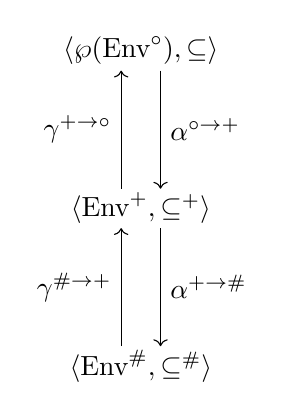
\begin{tikzpicture}[node distance=2cm]
\node (envcirc) {\(\langle\wp(\envcirc), \subseteq\rangle\)};
\node (envplus) [below of=envcirc] {\(\langle\envplus, \subseteq^{+}\rangle\)};
\node (envsharp) [below of=envplus]{\(\langle\envsharp, \subseteq^{\#}\rangle\)};

\draw [->] (.25,-0.25) -- (.25,-1.75) node[midway, right] {\(\alpha^{\circ\rightarrow +}\)};
\draw [->] (-.25,-1.75) -- (-.25,-0.25) node[midway, left] {\(\gamma^{+ \rightarrow\circ}\)};
\draw [->] (.25,-2.25) -- (.25,-3.75) node[midway, right] {\(\alpha^{+ \rightarrow\#}\)};
\draw [->] (-.25,-3.75) -- (-.25,-2.25) node[midway, left] {\(\gamma^{\# \rightarrow +}\)};
\end{tikzpicture}
\]

Uno \textit{stato} \(s^{\circ}\in\statecirc\triangleq\textrm{ProgramPoint}\times\envcirc\) è una coppia \(\langle pp, e^{\circ}\rangle\) formata da un \(pp\in\textrm{ProgramPoint}\) ed un \(e^{\circ}\in\envcirc\).

Una \textit{funzione di transizione} \(\tau\in\statecirc\rightarrow\statecirc\) è una funzione che indica come si susseguono gli stati durante l'esecuzione di un programma (può essere vista come la funzione che specifica la semantica di un programma). 

Un programma P è una coppia \(\langle\tau, \statecirc_{\textrm{init}}\rangle\in\textrm{Prog}\), dove:
\[\textrm{Prog}\triangleq [\statecirc\rightarrow\statecirc]\times\wp(\statecirc)\] 
Un programma è quindi formato da una funzione di transizione \(\tau\) e un insieme \(\textrm{State}^{\circ}_{\textrm{init}}\subseteq\statecirc\) di stati iniziali. 

Data un programma \(\textrm{P}=\langle\tau, \statecirc_{\textrm{init}}\rangle\in\textrm{Prog}\) possiamo definire l'insieme di \textit{tracce di esecuzione} di P come:

\[\Theta^{\circ}\llbracket\textrm{P}\rrbracket\triangleq\{\sigma\in(\statecirc)^{\ast}\ |\ \forall\ 0\leq i\leq |\sigma|-1.\ \tau(\sigma_i)=\sigma_{i+1}\}\]

Solitamente siamo interessati solo a un particolare sottoinsieme di tracce, ovvero quelle che partono da un stato iniziale \(s^{\circ}_{i}\in\textrm{State}^{\circ}_{\textrm{init}}\). L'insieme di tracce di esecuzione di P che iniziano con uno stato iniziale sono:

\[\Theta^{\circ}_i\llbracket\textrm{P}\rrbracket\triangleq\{\sigma\in(\statecirc)^{\ast}\ |\ \forall\ 0\leq i\leq |\sigma|-1.\ \tau(\sigma_i)=\sigma_{i+1} \wedge \sigma_0\in\statecirc_{\textrm{init}}\}\]

Possiamo ora definire l'insieme di stati raggiungibili da un programma P come:

\[\mathbb{S}\llbracket\textrm{P}\rrbracket\triangleq\{s\in\statecirc\ |\ \exists\ \sigma_1\cdot s\cdot \sigma_2\in\Theta^{\circ}_i\llbracket\textrm{P}\rrbracket.\ |\sigma_1|\geq 0 \wedge |\sigma_2|\geq 0\}\]

L'insieme di stati raggiungibili da un programma P, ovvero \(\mathbb{S}\llbracket\textrm{P}\rrbracket\), visto che non ci interessa l'ordine con cui questi stati vengono eseguiti, può anche essere visto come una funzione che mappa ogni \(pp\in\textrm{ProgramPoint}\) a un insieme \(env^{\circ}\in\wp(\envcirc)\) di environment. Ovvero il risultato di  \(\mathbb{S}\llbracket\textrm{P}\rrbracket\) può essere trasformato in un \(\cvcirc\) senza perdita di informazione (ovvero esiste una funzione biettiva  \(f:\wp(\statecirc)\rightarrow\cvcirc\)).

Definiamo ora un semplice linguaggio di programmazione basato su grafi che ci permetterò di fare un esempio concreto di interpretazione astratta (basandoci sul lavoro di Cousot del 1977). In questo linguaggio, che chiameremo CFG, un programma \(p\) è una coppia \(\langle\textrm{Nodes}, \textrm{Edges}\rangle\) formato da un insieme di nodi \(\textrm{Nodes}\subseteq\textrm{AllNodes}\) e un insieme di archi \(\textrm{Edges}\subset\textrm{AllEdges}\triangleq\textrm{Nodes}\times\textrm{Nodes}\) che collegano i nodi (con la condizione che: \(\forall \langle n_1, n_2\rangle\in \textrm{Edges} :n_1, n_2\in \textrm{Nodes} \wedge n_1\neq n_2\), ovvero ogni arco di un programma \(p\) deve collegare due nodi di \(p\) e un arco non può essere un autoanello di un nodo). L'insieme Edges si partiziona in tre sottoinsiemi disgiunti: TrueEdges, FalseEdges, SequentialEdges \(\subset\) Edges. L'insieme Nodes si partiziona in 5 sottoinsiemi disgiunti: Entry, Exit, Test, Assignment, Junctions \(\subset\) Nodes.

Definiamo alcune funzioni per un programma \(p=\langle\textrm{Nodes}, \textrm{Edges}\rangle\) (supponendo \(n \in\textrm{Nodes}\)):
\begin{align*}
origin,end :\ &\textrm{Edges}\rightarrow\textrm{Nodes}\ | \\
&\forall\ edge\in\textrm{Edges}, edge=\langle origin(edge), end(edge)\rangle \\
nodesSucc :\ &\textrm{Nodes}\rightarrow\wp(\textrm{Nodes})\ | \\
&nodeSucc(n)=\{n'\in\textrm{Nodes}\ |\ \exists\ edge\in\textrm{Edges}.\ edge=\langle n, n'\rangle\} \\
nodesPred :\ &\textrm{Nodes}\rightarrow\wp(\textrm{Nodes})\ | \\
&nodeSucc(n)=\{n'\in\textrm{Nodes}\ |\ \exists\ edge\in\textrm{Edges}.\ edge=\langle n', n\rangle\} \\
nodesSuccTrue :\ &\textrm{Test}\rightarrow\textrm{Nodes}\ | \\
&nodeSuccTrue(n)=\\
&=\{n'\in\textrm{NodesTrue}\ |\ \exists\ edge\in\textrm{Edges}.\ edge=\langle n, n'\rangle\} \\
nodesSuccFalse :\ &\textrm{Test}\rightarrow\textrm{Nodes}\ | \\
&nodeSuccFalse(n)=\\
&=\{n'\in\textrm{NodesFalse}\ |\ \exists\ edge\in\textrm{Edges}.\ edge=\langle n, n'\rangle\} \\
\end{align*}


Definiamo ora due funzioni che ci permetteranno di dire quali sono i nodi predecessori e quali sono i nodi successori di un nodo \(n\in nodes_p\):
\[nSucc:\]

Creiamo una partizione sull'insieme Nodes che distinguerà alcune categorie di nodi
\end{document}